\documentclass{scrartcl}
\author{Ronja Wagner, Clemens Tiedt}
\usepackage{amsfonts, amsmath, tikz}
\title{Mathematik II \\ Das Skript in verständlich}

\begin{document}

\maketitle
\pagebreak

Dieses Skript erhebt keinen Anspruch auf Vollständigkeit oder Richtigkeit, sondern hat zum Ziel, das existierende Skript von Dr. Börner zu ergänzen.
\pagebreak

\tableofcontents
\pagebreak

\section{Algebraische Strukturen}

\subsection{Allgemeine Definitionen}

%Hier vorher am liebsten nochmal eine allgemeinere Erläuterung zu Algebren: Was ist das und kann man das essen? bzw wozu brauchen wir das, was haben wir davon, irgendeine Menge mit Operationen zusammenzuklatschen?
Einer der wichtigsten Begriffe dieser Vorlesung ist die \emph{algebraische Struktur}. Um eine Struktur $\underline{A}$ zu definieren, benötigen wir zwei Bestandteile:

\begin{itemize}
    \item Eine Trägermenge $A$
    \item Operationen $f_1, f_2, ... f_n$, die auf dieser Trägermenge definiert sind
\end{itemize}

Die Trägermenge kann zuerst einmal eine beliebige nichtleere Menge sein. Häufig betrachten wir eine Menge von Zahlen (z.B. $\mathbb{N}$ oder $\mathbb{Z}$),
aber wir können genau so gut eine Algebra der Kekse oder eine der Farben definieren. 

Eine Operation\footnote{Definition 13.1} auf $A$ definieren wir als Abbildung, die $n$ Elemente der Menge $A$ verknüpft und auf ein anderes Element aus $A$ abbildet. Mathematisch schreiben wir das als $f: A^n \to A$
- die Operation $f$ ordnet also je $n$ Elementen aus $A$ einen "Funktionswert" aus $A$ zu.
Operationen sind eigentlich nur eine abstraktere und allgemeinere Beschreibung von etwas, das wir bereits aus der Grundschule kennen - so ist z. B. das + einfach eine Operation, die zwei reellen Zahlen eine dritte zuweist, formal nach unserer vorherigen Definition also $+: \mathbb{R}^2 \to \mathbb{R}$. Ein Beispiel für eine Operation von Grad 3 wäre der Flächeninhalt einer Pyramide mit rechteckiger Grundfläche, die Länge, Breite und Höhe den Flächeninhalt zuweisen.
%ZWEISTELLIGE:
Für Operationen nutzen wir normalerweise nicht die Funktionsschreibweise $\circ(a, b)$, sondern $a \circ b$.
%Farbmischung am besten hier schon einführen

Operationen können beliebige Stelligkeit besitzen, d.h. beliebig viele Elemente verknüpfen. Meist betrachten wir zweistellige ("binäre") Operationen, da wir diese auf beliebige
Stelligkeit erweitern können.
%Hier auf jeden Fall noch Beispiele für mehrstellige und einstellige Operationen einbauen, außerdem Konstanten, da das Konzept Kontante = Funktion ohne Parameter evtl etwas schwierig ist

Weiterhin definieren wir für Operationen die Abgeschlossenheit\footnote{Definition 13.2}. Wir bezeichnen eine \emph{Menge} $B \subseteq A$ als abgeschlossen unter einer Operation $f: A^n \to A$,
wenn das Bild von $f$ Teilmenge von B ist.
%Hier noch zu kompliziert
Anders ausgedrückt verlassen wir die Menge $B$ nie, indem wir $f$ auf Elemente von $B$ anwenden. Ist $B \subseteq A$ unter $f$ abgeschlossen, 
können wir die Einschränkung $f|_ B$ von $f$ auf $B$ definieren, welche die Operation $f$ nur noch für den Definitions- und Wertebereich $B$ definiert.

Nun haben wir alle Bausteine, um den Begriff der \emph{(universellen) Algebra} zu definieren. Bestehend aus

\begin{itemize}
    \item einer Trägermenge $A$ (meist mit $A \ne \emptyset$)
    \item Operationen $f_1, f_2, ..., f_n$
    \item Konstanten\footnote{Eine Konstante ist eine Operation ohne Parameter, also eine Abbildung $c: \emptyset \to A$, die auf ein $c \in A$ zeigt} $c_1, c_2, ..., c_n$
\end{itemize}

bezeichnen wir $\underline{A} = \langle A; f_1, f_2, ..., f_n; c_1, c_2, ..., c_n \rangle$ als universelle Algebra. Falls die Konstanten eindeutig oder nicht von Interesse sind,
können sie häufig auch weggelassen werden.

\subsection{Unteralgebren und Erzeugendensysteme}

\paragraph{Unteralgebren}
Häufig betrachten wir statt einer kompletten Struktur eine Teilstruktur, z.B. können wir die ganzen Zahlen $\langle \mathbb{Z}; + \rangle$ auf die natürlichen Zahlen
$\langle \mathbb{N}; + \rangle$ einschränken. Die natürlichen Zahlen mit der Addition sind eine Unterstruktur der ganzen Zahlen, weil sie unter der Addition abgeschlossen sind.
Bei der Addition zweier positiver Zahlen kann nie eine negative Zahl herauskommen. Allgemein ist die Struktur $\underline{B}$ Unterstruktur von $\underline{A}$, wenn die
Trägermenge $B \subseteq A$ ist und $B$ auch unter den Operationen $f_1, f_2, ..., f_n$ auf $A$ abgeschlossen ist und alle Konstanten $c_1, c_2, ..., c_n \in A$ auch in $B$
enthalten sind. Dann schreiben wir $B \le A$.    


\paragraph{Erzeugendensysteme}
Als nächstes widmen wir uns Erzeugendensystemen. Hierzu betrachten wir eine Struktur $\underline{A}$ und eine Menge $C \subseteq A$. Wir wenden nun auf $C \cup \{c_1, c_2, ..., c_n\}$
die Operationen $f_1, f_2, ..., f_n$, die auf $A$ definiert sind, an und nehmen die $f(c) \in A, c \in C$ in die Menge $C$ auf. Wir erweitern die Menge $C$ also um alle Elemente, die wir
durch wiederholtes Anwenden der Operationen von $\underline{A}$ erzeugen können. Ist die Algebra $\langle C \rangle = \underline{A}$, bezeichnen wir $C$ als \emph{Erzeugendensystem} von 
$\underline{A}$.

\subsection{Spezielle Strukturen}

Es haben sich einige Strukturen mit besonderen Eigenschaften etabliert, die wir hier einführen wollen. Die erste ist die \emph{Halbgruppe}.

\paragraph{Halbgruppen}
Eine Halbgruppe ist eine Struktur $\langle H; \circ \rangle$, wobei $\circ$ eine zweistellige Operation ist und für die das Assoziativgesetz gilt, d.h. für $a, b \in H$:
%Ich wäre eher dafür, zuerst die verständliche und dann die mat

\begin{equation*}
    (a \circ b) \circ c = a \circ (b \circ c) = a \circ b \circ c
\end{equation*}

Ein Beispiel ist die additive Farbmischung. Wenn wir $F$ als Menge der Farben definieren und $\circ$ als das Mischen zweier Farben, so ist ersichtlich, dass es keinen Unterschied macht,
ob wir bei der Mischung dreier Farben zuerst z.B. Rot mit Blau und das Ergebnis mit Gelb oder Rot mit der Mischung von Blau und Gelb mischen. Tatsächlich spielt hier sogar die Reihenfolge
keine Rolle, womit die Halbgruppe der additiven Farbmischung eine weitere Eigenschaft erfüllt: Sie ist kommutativ.

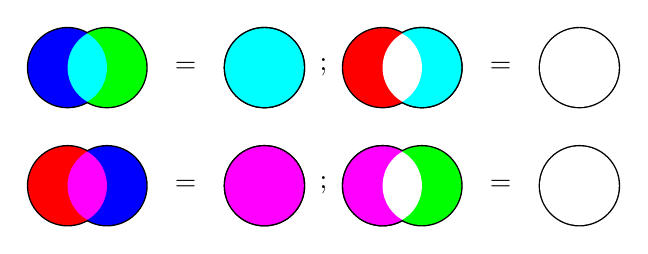
\begin{tikzpicture}[blend group=screen]
    \draw [fill={rgb: red,255;green,0;blue,0}] (2, 0) circle (0.5);
    \draw [fill={rgb: red,0;green,0;blue,255}] (2.5, 0) circle (0.5);
    \draw (3.5, 0) node {=};
    \draw [fill={rgb: red,255;green,0;blue,0}] (4.5, 0) circle (0.5);
    \draw [fill={rgb: red,0;green,0;blue,255}] (4.5, 0) circle (0.5);
    \draw (5.25, 0) node {;};
    \draw [fill={rgb: red,255;green,0;blue,0}] (6, 0) circle (0.5);
    \draw [fill={rgb: red,0;green,0;blue,255}] (6, 0) circle (0.5);
    \draw [fill={rgb: red,0;green,255;blue,0}] (6.5, 0) circle (0.5);
    \draw (7.5, 0) node {=};
    \draw [fill=white] (8.5, 0) circle (0.5);

    \draw [fill={rgb: red,0;green,0;blue,255}] (2, 1.5) circle (0.5);
    \draw [fill={rgb: red,0;green,255;blue,0}] (2.5, 1.5) circle (0.5);
    \draw (3.5, 1.5) node {=};
    \draw [fill={rgb: red,0;green,0;blue,255}] (4.5, 1.5) circle (0.5);
    \draw [fill={rgb: red,0;green,255;blue,0}] (4.5, 1.5) circle (0.5);
    \draw (5.25, 1.5) node {;};
    \draw [fill={rgb: red,255;green,0;blue,0}] (6, 1.5) circle (0.5);
    \draw [fill={rgb: red,0;green,0;blue,255}] (6.5, 1.5) circle (0.5);
    \draw [fill={rgb: red,0;green,255;blue,0}] (6.5, 1.5) circle (0.5);
    \draw (7.5, 1.5) node {=};
    \draw [fill=white] (8.5, 1.5) circle (0.5);
\end{tikzpicture}


Allgemein heißt eine Halbgruppe $H$, in der für $a, b \in H$ die Beziehung $a \circ b = b \circ a$ gilt \emph{kommutative} oder \emph{abelsche} Halbgruppe.

\paragraph{Neutrale Elemente}
Manche Halbgruppen $\langle H; \circ \rangle$ enthalten besondere Elemente $e \in H$, die bezogen auf die Operation $\circ$ "nichts tun". Ein klassisches Beispiel ist für $\langle \mathbb{N}; + \rangle$
die 0. Nehmen wir bei den Farben noch die Transparenz als Eigenschaft hinzu, ist die vollkommen transparente Farbe ein Nullelement.

Allgemein ist ein Element $e \in H$ neutrales Element, wenn für alle $a \in H$ gilt:

\begin{equation*}
    e \circ a = a \circ e = a
\end{equation*}

\paragraph{Monoiden}
Enthält eine Halbgruppe $\langle H; \circ \rangle$ ein neutrales Element $e$ bezeichnen wir sie als Monoid $\langle H; \circ; e \rangle$. Innerhalb eines Monoiden $\langle H; \circ; e \rangle$
können wir nun den Begriff des Inversen definieren. Für ein Element $a \in H$ ist $x \in H$ ein inverses Element, wenn $x \circ a = a \circ x = e$ gilt. Anschaulicher gesprochen heben sich die 
Elemente $a$ und $x$ durch die Operation $\circ$ auf.

KEkse!!!!

\end{document}